\section{Evaluation}
\label{sec:evaluation}

The graph analyzed consisted of seven edge types, $N_1=10^4, N_2=10^5, N_3=10^6, N_4=10^7,  N_5=10^8, N_6=10^9, N_7=10^{10}$, totaling 11 billion edges, with access probabilities $p_1 =0.5, p_2 =0.25, p_3=0.13, p_4=0.06, p_5=0.03, p_6=0.02$ and $p_7 =0.01$; a graph of this size would have approximately 1 billion vertices.
The number of read operations per query is geometrically distributed starting at $2$, with an average of $15$, before a write.
In all edge types, a fraction $0.3$ are distributed, the remainder are local; in proportion with a good graph partitioning algorithm.
The delay $d$ between a transaction completing a tentative write at one end and starting at another end is exponential distributed with a mean of $5ms$.
The database is initial clean and considered to be corrupted when $10$\% ($\gamma = 0.1$) of all edges are corrupted.
The time taken until operational corruption $U$, is measured in days.
$U$ considered for a range of transaction arrival rates, $\lambda = (1000, ..., 10000)$; a typical graph workload comprises of 90\% read-only transactions and 10\% read-write transactions \cite{Angles2020}, hence the chosen range reflects a total workload of $\lambda = (10000, ..., 100000)$.
The following $\Delta$ values were considered $\Delta = 50, 75, 100ms$.
For each $\Delta$ the probability that $d$ exceeds $\Delta$ is $P(D > \Delta) = 4.5 \time 10^{-5}, 3.1 \times 10^{-7}, 2.1 \times 10^{-9}$ respectively.

The results for measuring the impact of $\Delta$ on the time until operational corruption are given in Figure \ref{time-to-corruption-results}.
Under no isolation, $U$ ranges between 50-500 days.
For $50ms$ this increases to 1-75 years. For $\Delta = 75, 100ms$ the time to corruption vastly exceeds lifetime of any system making data corruption resulting from half-corrupted edges of little practical concern.

\begin{figure}[h]
  \centering
  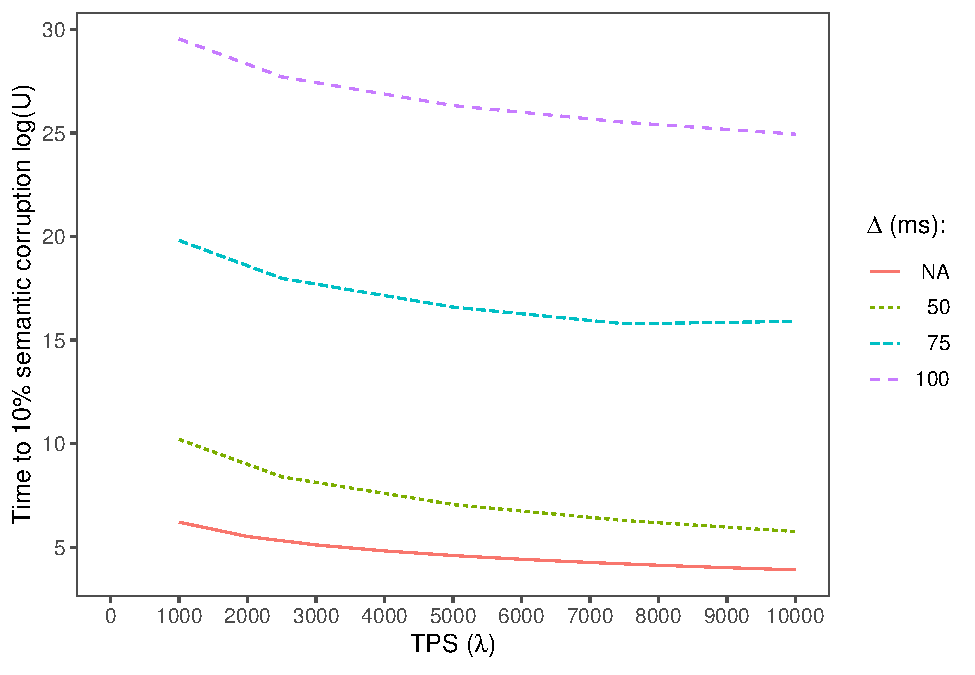
\includegraphics[width=\linewidth]{./figures/delta}
  \caption{Time until operational corruption.}
  \label{time-to-corruption-results}
\end{figure}

The number of aborts per second for $\Delta = 50, 75, 100ms$ are given in Figure \ref{aborts-results} for the most popular edge type, $N=10^4$. The simulation was ran for 10 seconds for a range of transaction arrival rates, $\lambda = (1000, ..., 10000)$. For $\Delta = 50$ the abort rate varies between $1-5\%$, this increases to between $1-7\%$ and $1-9\%$ for $\Delta = 75$ and $\Delta = 100$ respectively.

\begin{figure}[h]
  \centering
  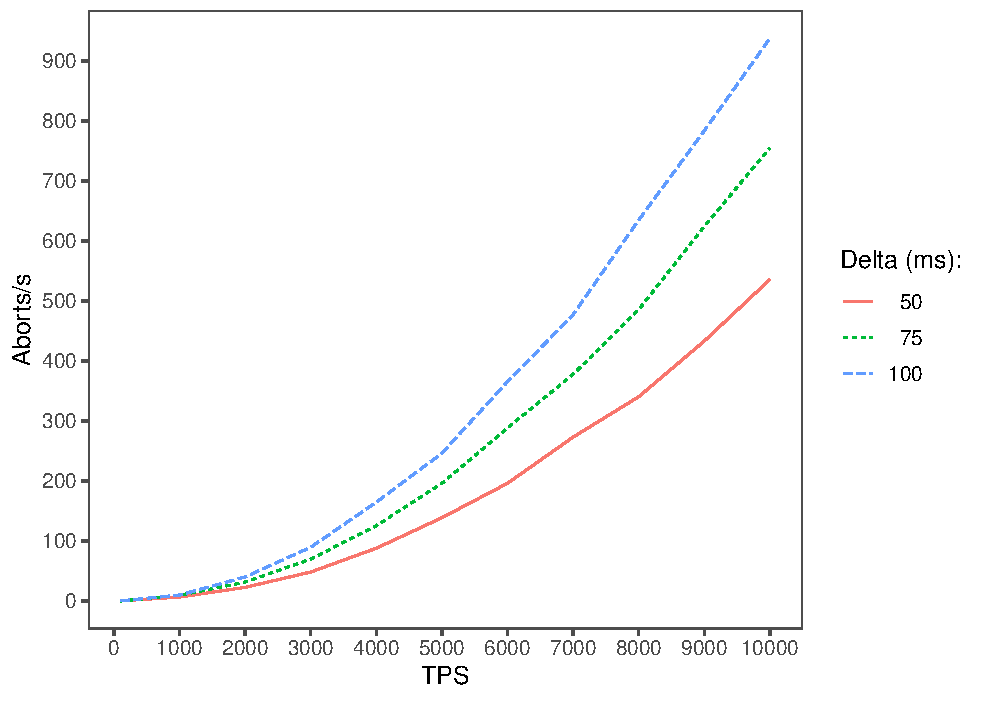
\includegraphics[width=\linewidth]{./figures/aborts}
  \caption{Number of aborts per second.}
  \label{aborts-results}
\end{figure}
